\begin{apendicesenv}

\partapendices

\chapter{Primeiro Apêndice}
\label{app:pessoas}
\begin{figure}[H]
	\centering
    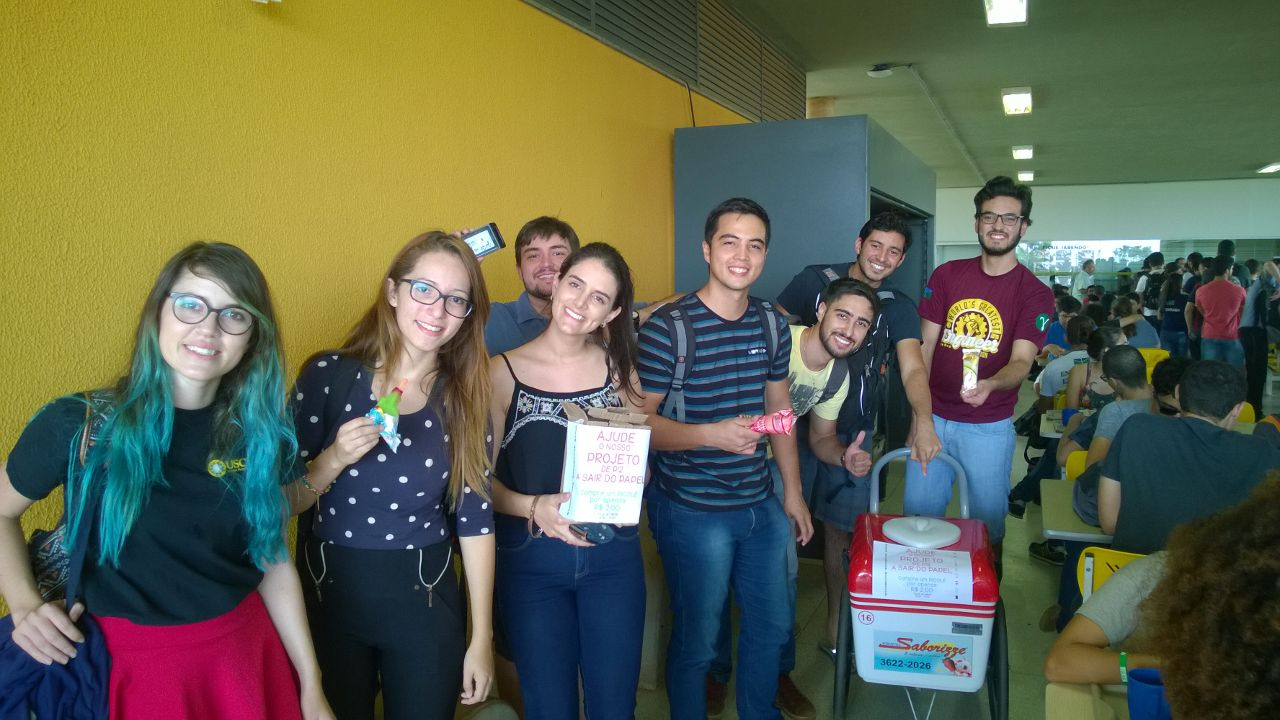
\includegraphics[scale=0.5]{figuras/pessoas}
    \caption{Equipe parcial do $\pi col\acute{e}$ durante a venda de picolés na FGA no dia 24 de março de 2017. }
    \label{fig:fotopessoas}
\end{figure}

A figura \ref{fig:fotopessoas} comprova o primeiro trabalho realizado para a integração e engajamento da equipe. A venda de picolé na FGA deu-se no intuito de arrecadar dinheiro para o projeto, aproximar a equipe, realizar medicões de temperatura e também de uma análise de demanda.

\chapter{Segundo Apêndice}

	Experimento realizado na FGA, no dia 24.03 com início às 12:25;

Condições Iniciais:
     	Temperatura: 30,6º e
     	Umidade: 35\%
        
        \begin{figure}[H]
	\centering
    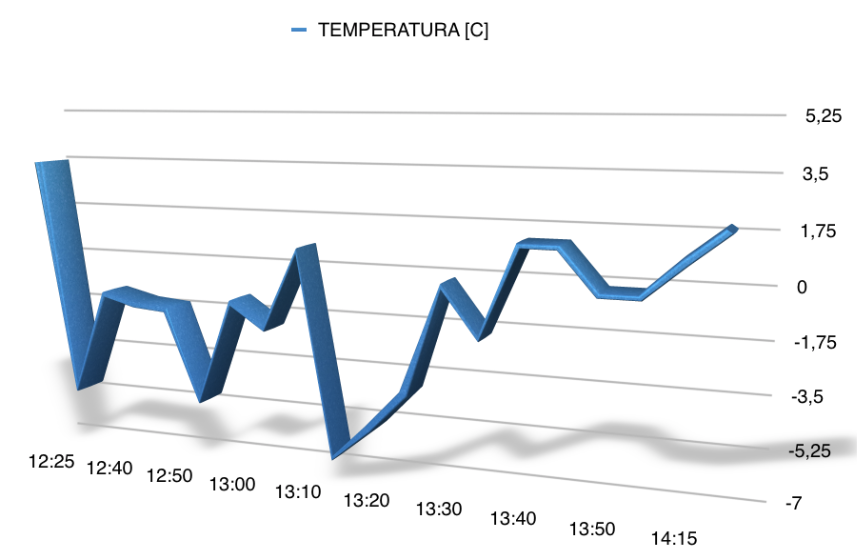
\includegraphics[width=\textwidth]{figuras/temperatura}
    \caption{Tempo x Temperatura}
    \label{fig:temperatura}
\end{figure}
	Com o gráfico, pode-se analisar o comportamento térmico, bem como a capacidade de regeneração da câmara fria em condições de venda. Inicialmente o resfriamento até a temperatura de trabalho, onde os materiais de forração ficam responsáveis pela redução das perdas de calor durante o trabalho, como também a relação das aberturas de tampa para pegar o picolé que representam a maior parte das perdas térmicas. O gráfico mostra de maneira clara o aumento da temperatura média em decorrer da redução dos picolés em seu interior, os quais também corroboram para manter a temperatura mais próxima do ideal.
	
      


\end{apendicesenv}
